\documentclass{../source/Experiment}

\major{信息工程}
\name{姚桂涛}
\title{集成运算放大器应用电路研究}
\stuid{3190105597}
\college{信息与电子工程学院}
\date{\today}
\lab{东4-216}
\course{电子电路设计实验}
\instructor{李锡华、施红军、叶险峰}
\grades{}
\expname{集成运算放大器应用电路研究}
\exptype{研究实验}
\partner{杜秉哲}

\begin{document}
    \makecover
    \makeheader

    \section{实验目的}
        \begin{enumerate}
            \item 学习和研究由集成运放构成的积分器、比较器、波形发生器等应用电路的组成与原理,掌握其设计方法。
            \item 观察积分运算电路在实际应用时存在的积分漂移、积分误差等现象,了解解决方法。
        \end{enumerate}
    \section{实验任务和要求}
        \subsection{反相积分器的设计研究}
            \begin{enumerate}
                \item 设计反相积分电路,方波→三角波。\\
                设计要求:\\
                方波:幅度$2.2V$、频率$500Hz$\\
                三角波:幅度$2V$左右
                \item 安装该电路,输入方波,用示波器双踪显示输入、输出波形,测量并记录波形,标示出各实测参数。
            \end{enumerate}
        \subsection{迟滞比较器设计研究}
            \begin{enumerate}
                \item 设计一迟滞比较器,使$V_{TH} \approx \frac{1}{2}(V_Z + V_D)$\\
                允许使用电阻值在$20k\Omega$~$400k\Omega$之间。
                \item 安装电路,输入$500Hz$三角波(幅度合理自定),	研究输入、输出信号的幅度、相位关系。
            \end{enumerate}
        \subsection{方波-三角波发生器研究}
            \begin{enumerate}
                \item 断开迟滞比较器信号输入,搭建方波-三角波发生电路,调节电位器$R_{w4}$,可产生不同频率方波、三角波。观察电压$V_{42o’}$与输出信号频率的关系,测量并记录可调频率范围。
            \end{enumerate}
    \section{实验方案设计与实验参数计算}
        \subsection{反相积分器的设计研究}
            电路图:\\
            \begin{figure}[h]
                \centering
                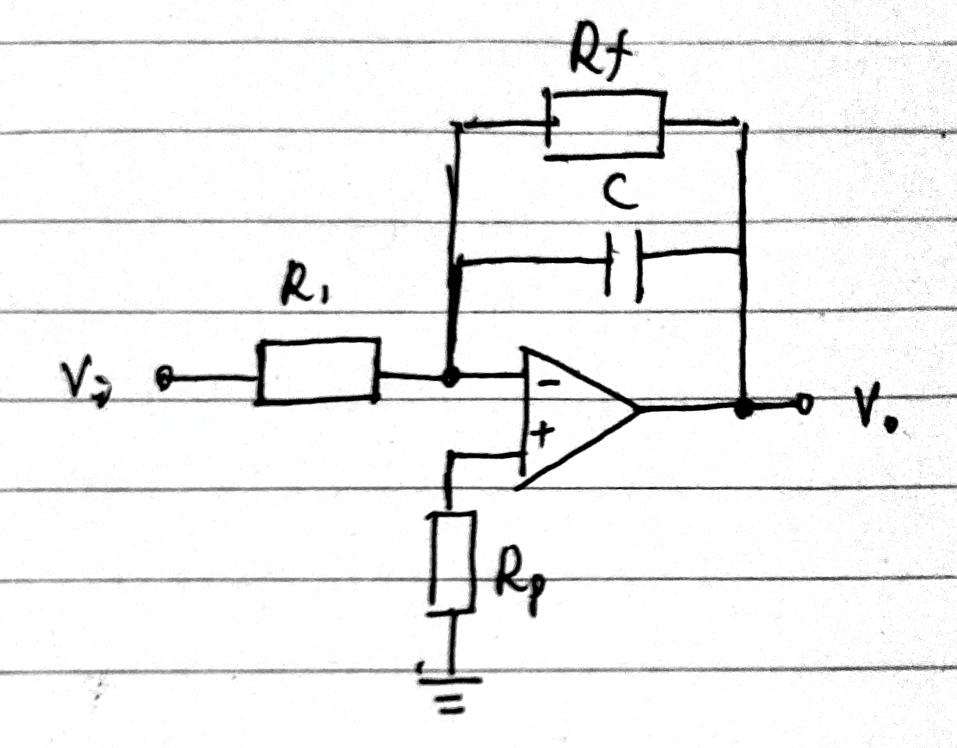
\includegraphics[width = 3in]{pic/集成2.png}
                \caption{设计电路图}
            \end{figure}

            参数计算:\\
            由
            $$2B = \frac{A}{R_1C}\frac{T}{2}$$
            已知$C = 0.22\mu F$,得$R_1 = 2.5k\Omega$,取标称值$R_1 = 2.4k\Omega$\\
            为消除积分漂移同时减小积分误差,通常取$R_f>10R_1$,所以取$R_f = 24k\Omega$    
        \subsection{迟滞比较器设计研究}
            电路图:\\
            \begin{figure}[h]
                \centering
                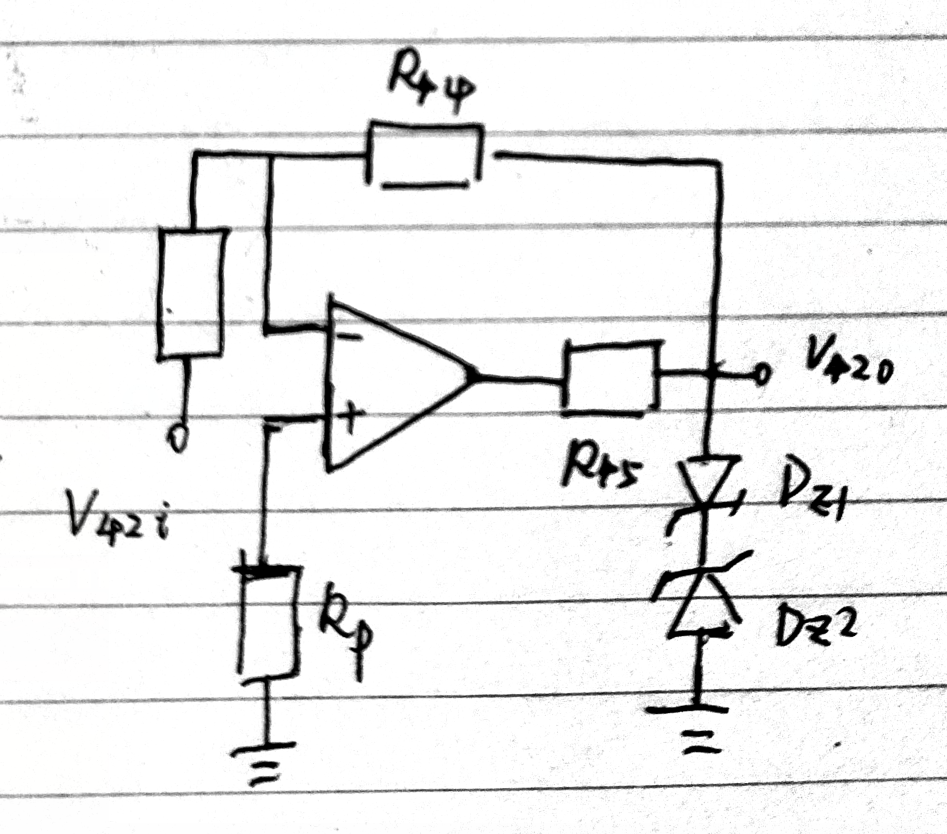
\includegraphics[width = 3in]{pic/集成3}
                \caption{设计电路图}
            \end{figure}

            参数计算:\\
            由
            $$V_{TH} = \frac{R_{43}}{R_{44}}(V_Z + V_D)$$
            同时因允许使用电阻值在$20k\Omega$~$400k\Omega$之间,取$R_{43} = 100k\Omega,\, R_{44} = 200k\Omega$。
        \subsection{方波-三角波发生器研究}
            电路图:\\
            \begin{figure}[h]
                \centering
                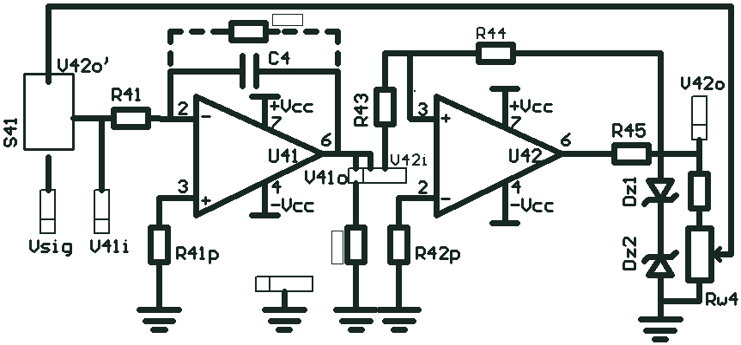
\includegraphics[width = 3in]{pic/集成1}
                \caption{设计电路图}
            \end{figure}
    \section{主要仪器设备}
        电路板、信号发生器、直流电源、示波器
    \section{实验步骤、实验调试过程、实验数据记录}
        \subsection{反相积分器的设计研究}
            安装该电路,输入方波,用示波器双踪显示输入、输出波形,测量并记录波形,标示出各实测参数。\\
            结果
            \begin{figure}[h]
                \centering
                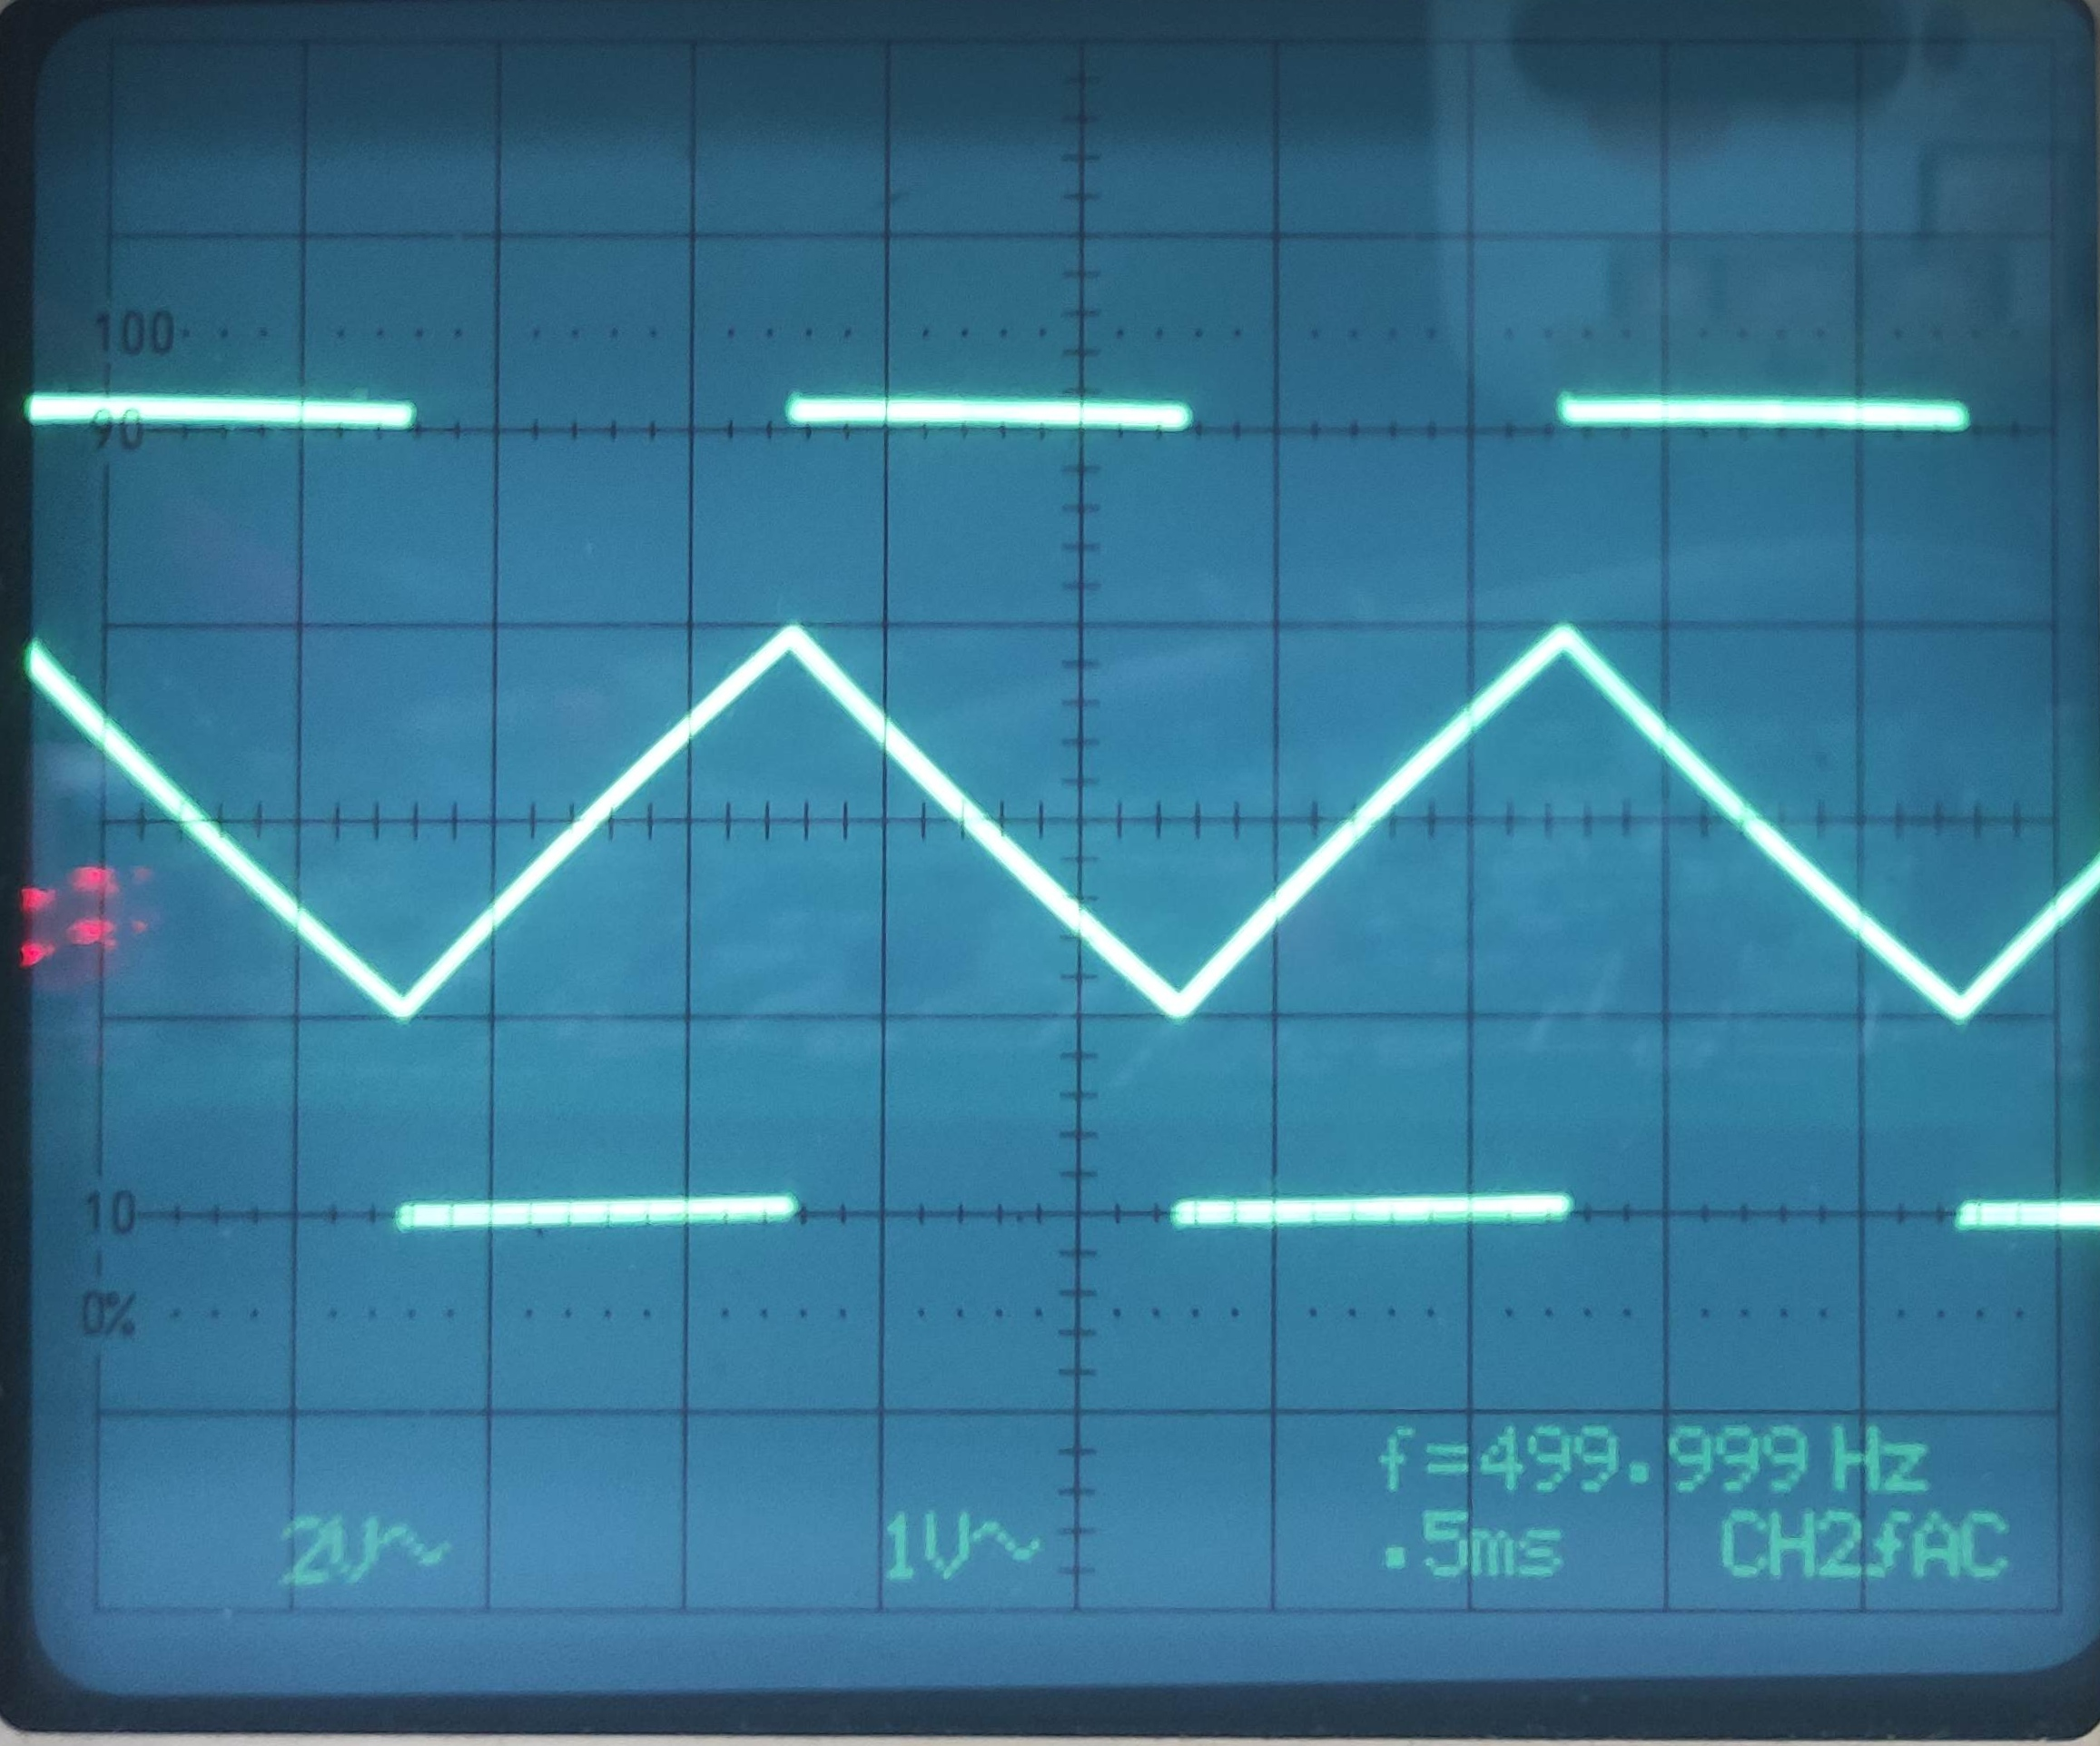
\includegraphics[width = 3in]{实验一2}
                \caption{实验1结果}
            \end{figure}
            测得:\\
            $V_i = 2.08V,\, V_o = 1.98V$
        \subsection{迟滞比较器设计研究}
            安装电路,输入$500Hz$三角波(幅度合理自定),研究输入、输出信号的幅度、相位关系。
            \begin{figure}[h]
                \centering
                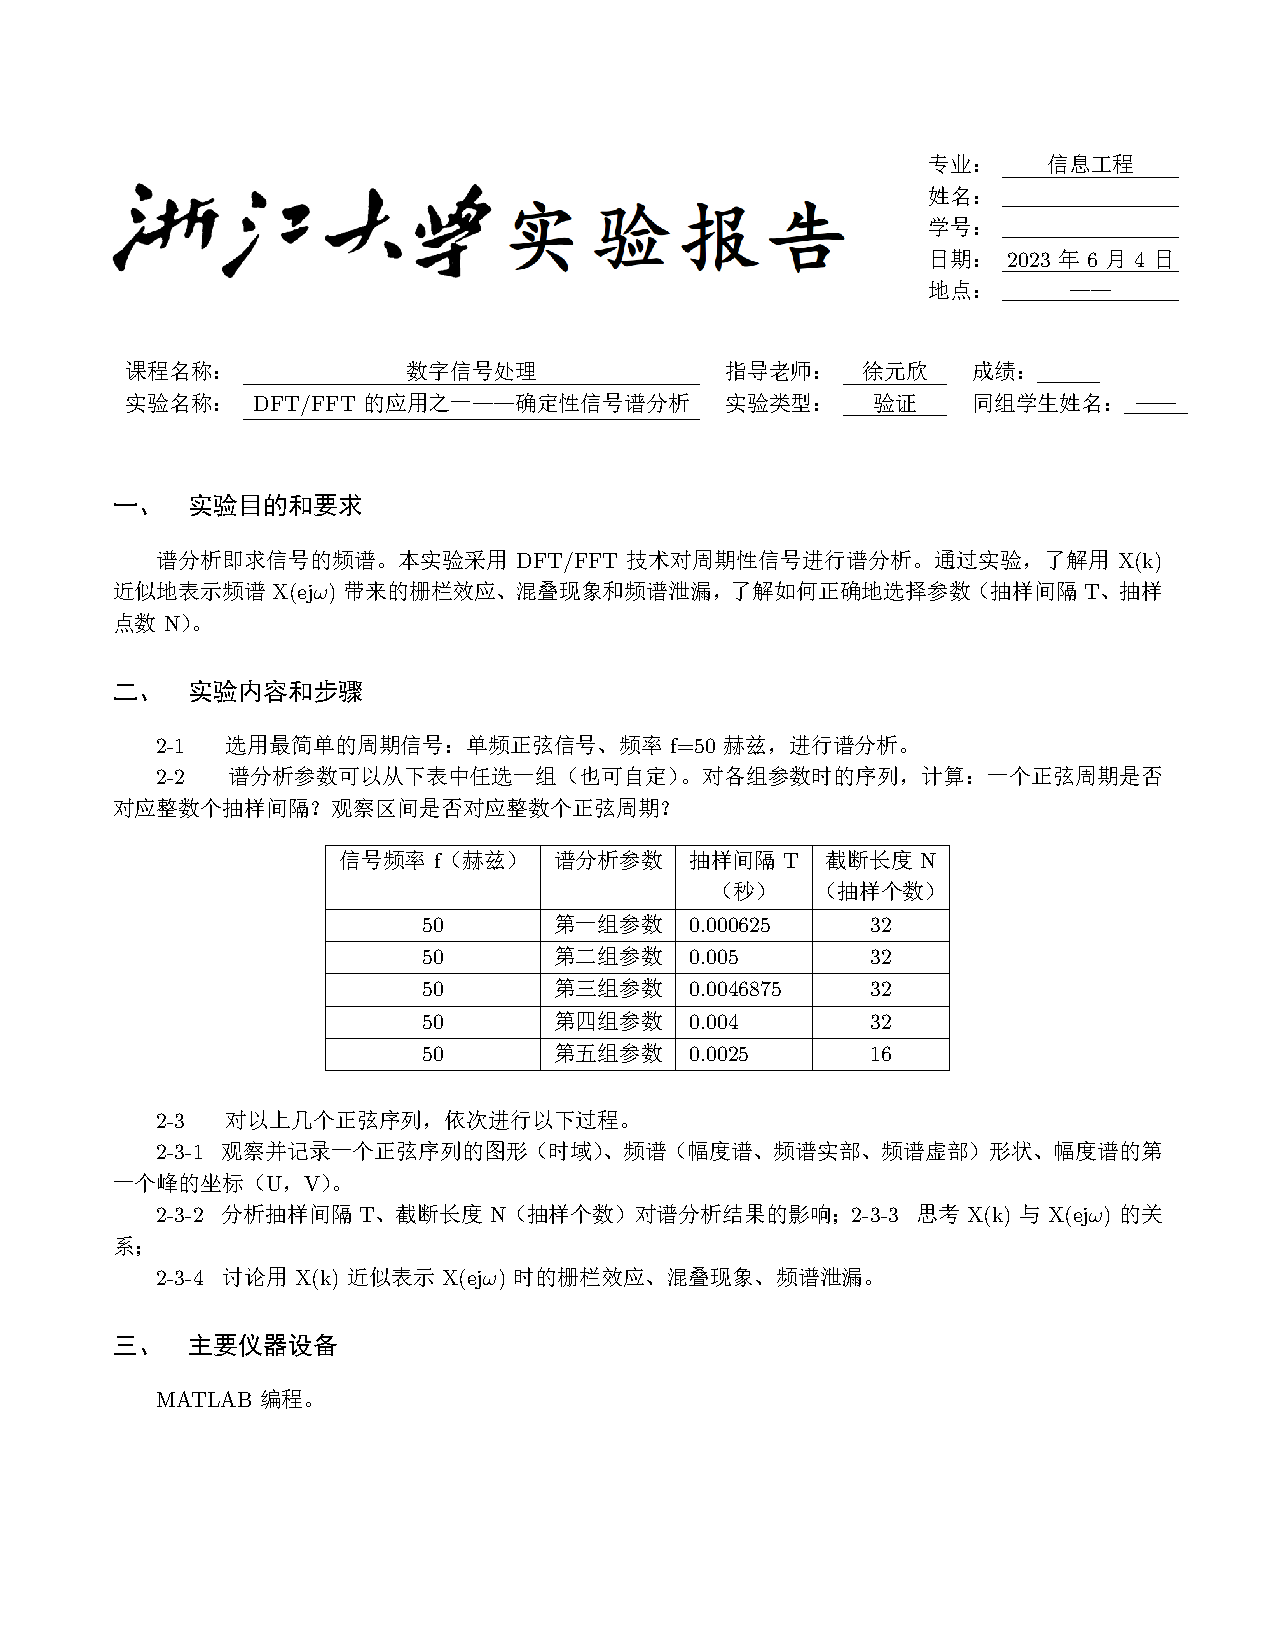
\includegraphics[width = 2.5in]{实验二}
                \caption{实验二结果}
            \end{figure}
            测得:\\
            $V_i = 6.28V,\, V_o =  (V_Z+V_D) = 6.88V,\, V_{TH} = 3.84V$ \\
            相位差:$\Delta \varphi = 34°34’$
        \subsection{方波-三角波发生器研究}
            断开迟滞比较器信号输入,搭建方波-三角波发生电路,调节电位器$R_{w4}$,可产生不同频率方波、三角波。观察电压$V_{42o’}$与输出信号频率的关系,测量并记录可调频率范围。\\
            结果: 
            \begin{table}[h]
                \centering
                \begin{tabular}{|c|c|}
                    \hline
                    $V_{42o’}$ & $f$         \\
                    \hline 
                    $1.28V$    & $174.407Hz$ \\
                    \hline 
                    $3.20V$    & $420.656Hz$ \\
                    \hline 
                    $4.80V$    & $628.634Hz$ \\
                    \hline 
                    $6.36V$    & $870.473Hz$ \\
                    \hline 
                \end{tabular}
            \end{table}

            调节$R_{w4}$,直到频率上限
            \newpage
            \begin{figure}[h]
                \centering
                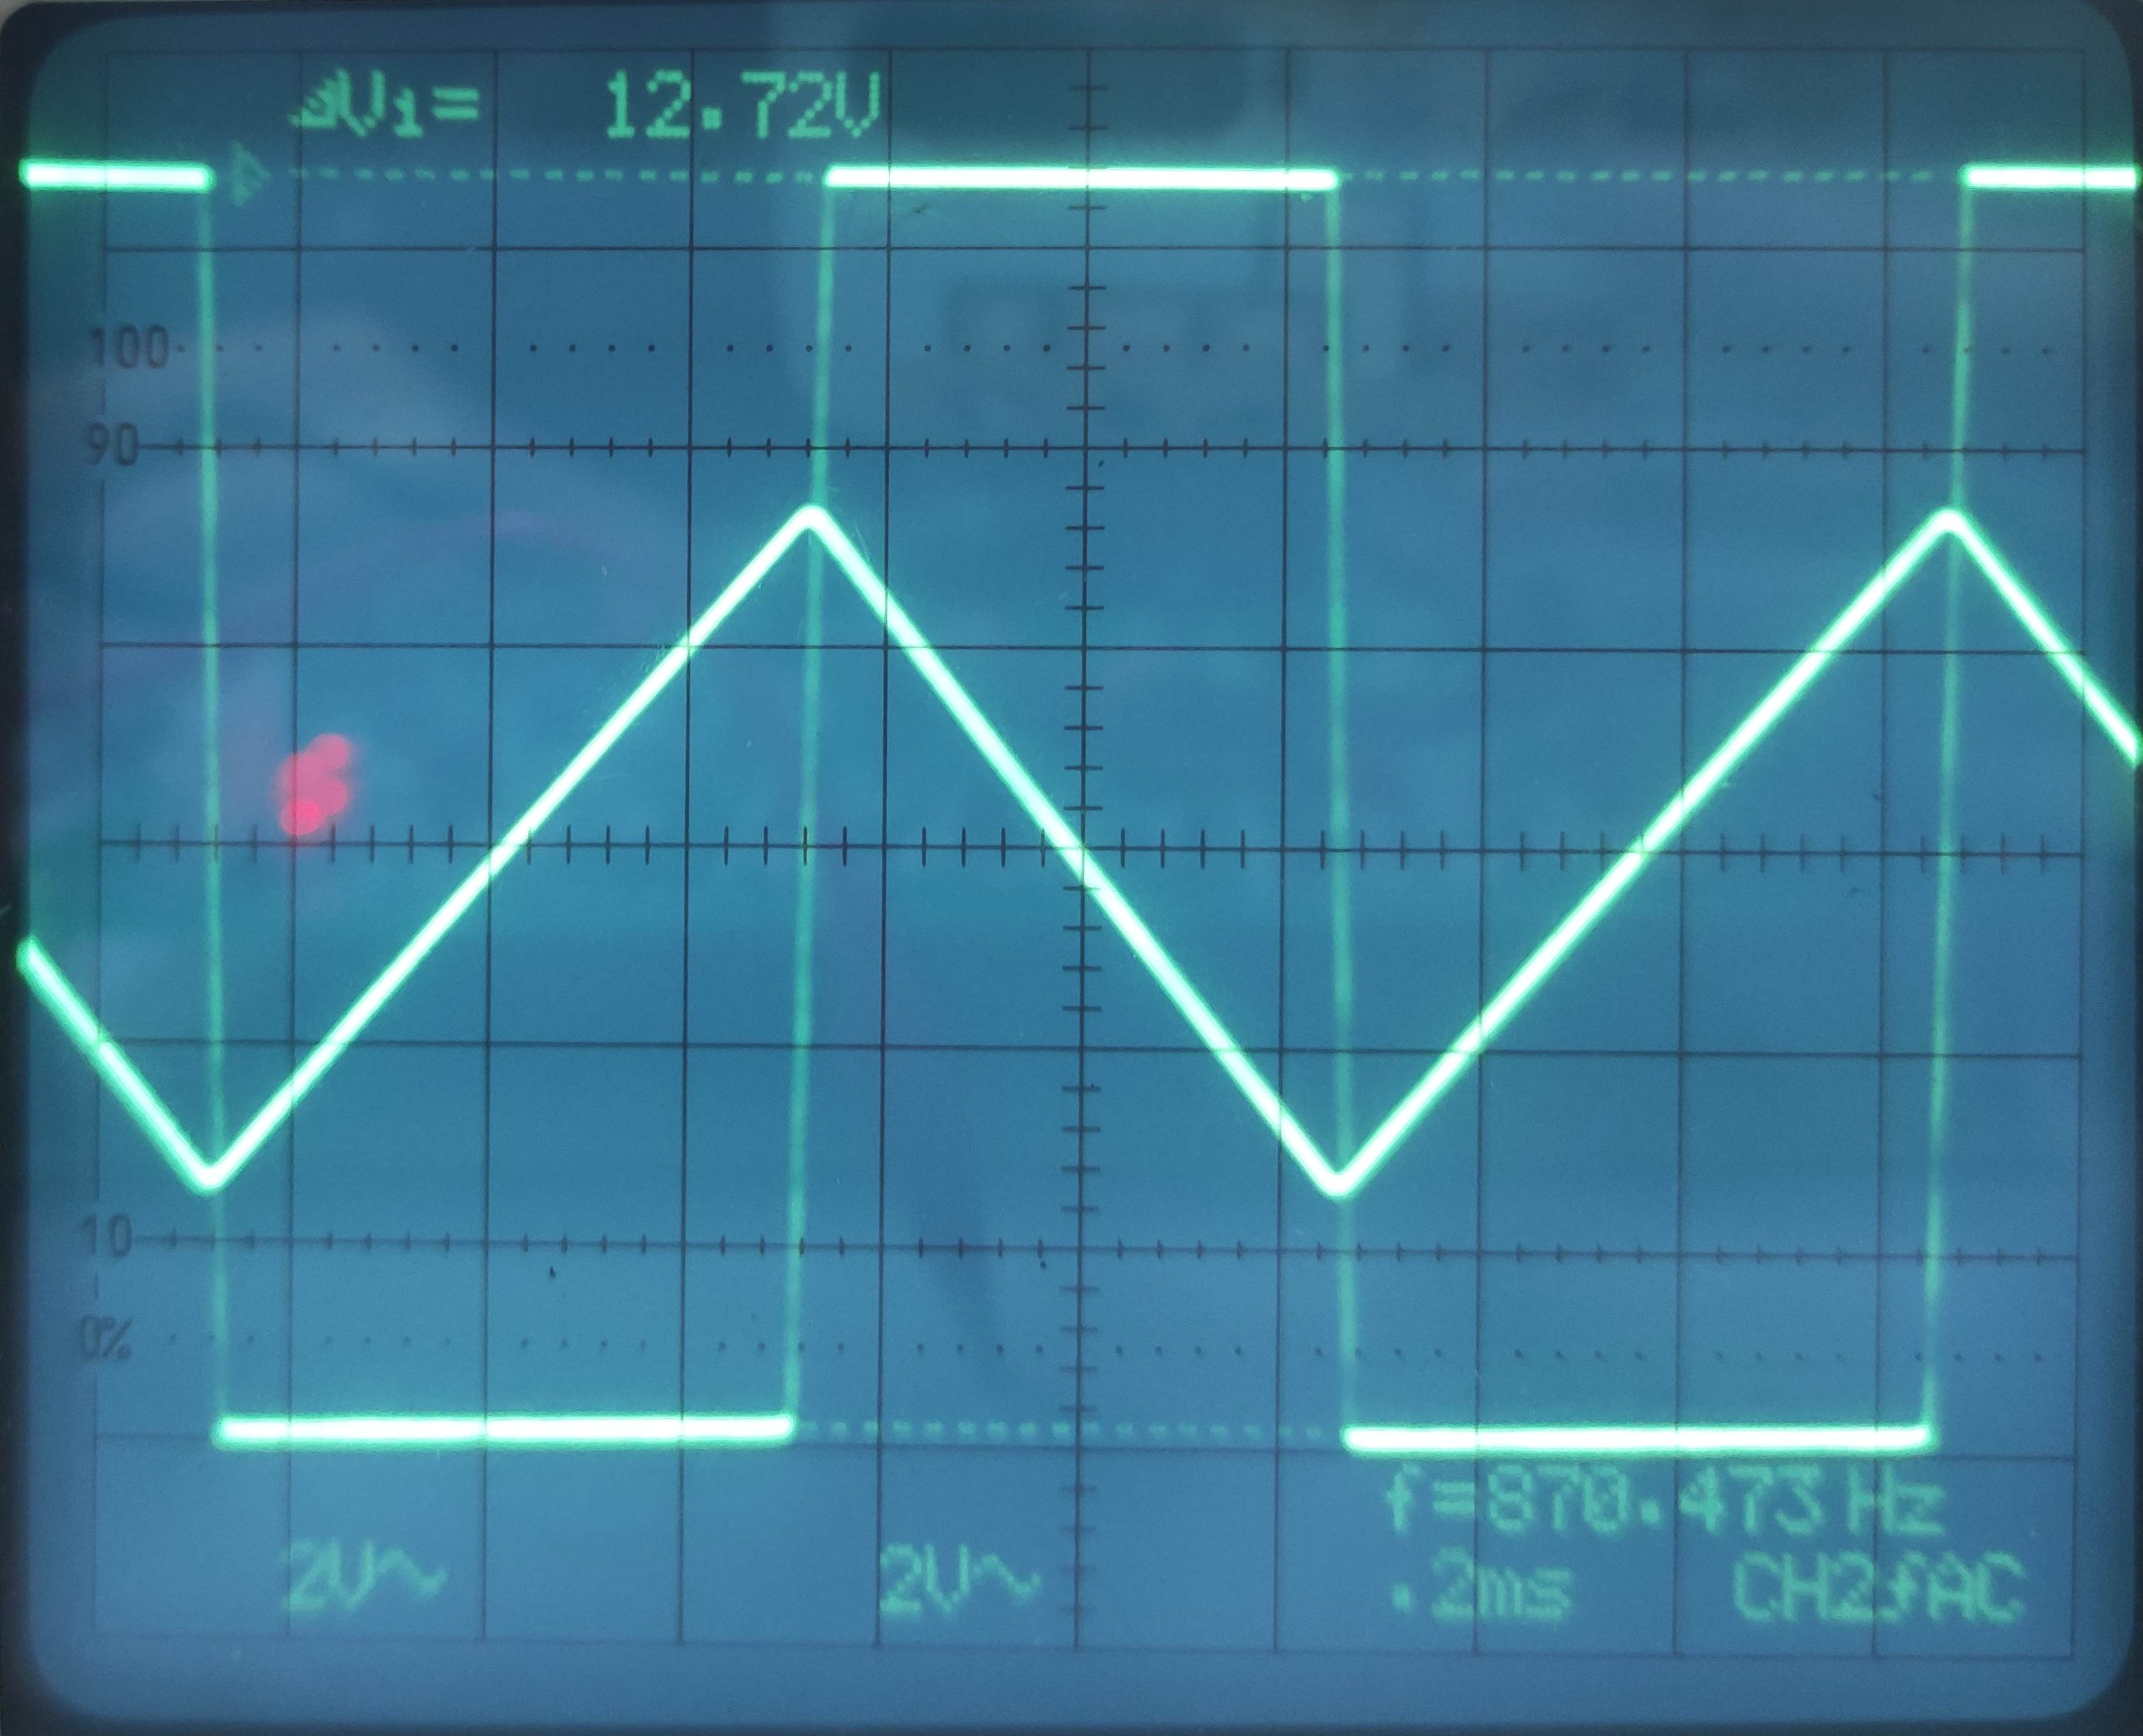
\includegraphics[width = 2.5in]{上限}
                \caption{频率上限}
            \end{figure}

            得到可调频率范围:$f \leq 870.420Hz$
    \section{实验结果和分析处理}
        \subsection{反相积分器的设计研究}    
        通过结果可以得到,在输入幅度为2.08V的方波信号时,输出为幅度为1.98V的三角波,基本符合设计要求。由于$R_1$理论计算值为$2.5k\Omega$,但是由于标称值只能取到$2.4k\Omega$,所以会导致一定的误差。
        \subsection{迟滞比较器设计研究}
        通过实验结果可以得到,$V_{TH} = 3.84V,\, \frac{1}{2}(V_Z + V_D) = 3.44V,\, V_{TH} \approx \frac{1}{2}(V_Z + V_D)$,所以满足设计要求。
        \subsection{方波-三角波发生器研究}
        由实验结果可以得到,$V_{42o’}$越高,输出信号的频率越高。同时,可调频率范围为$f \leq 870.420Hz$。
    \section{讨论、心得}
         通过本次实验,我对集成运放电路构成的积分器、比较器、波形发生器应用电路有了更深的理解。同时通过自主设计电路,掌握了其设计方法。
         也学会了如何解决积分运算电路在实际应用中存在的积分漂移、积分误差。
\end{document}